\documentclass[12pt,a4paper]{article}
\usepackage[margin=2cm]{geometry}
\usepackage{amsmath,amssymb}
\usepackage{graphicx}
\usepackage{fancyhdr}
\usepackage{array}
\usepackage{tikz}
\usepackage{enumitem}
\usepackage{tcolorbox}
\usetikzlibrary{arrows.meta}

% Header/Footer
\pagestyle{fancy}
\fancyhf{}
\fancyhead[L]{\textbf{\Large CONTOUR}\textsf{EDUCATION}}
\fancyhead[R]{Year 10 Mathematics}
\fancyfoot[L]{MA10 - Linear Equations Review - Mock CAT}
\fancyfoot[R]{\thepage}
\renewcommand{\headrulewidth}{0pt}
\renewcommand{\footrulewidth}{0pt}

% Question box environment
\newtcolorbox{questionbox}{
    colback=white,
    colframe=black,
    boxrule=0.5pt,
    arc=0pt,
    left=5pt,
    right=5pt,
    top=5pt,
    bottom=5pt
}

\begin{document}

% Title Page
\begin{center}
\vspace*{3cm}

{\Huge \textbf{\textsf{CONTOUR}}\textsf{EDUCATION}}

\vspace{0.5cm}
\small Website: contoureducation.com.au | Phone: 1800 888 300\\
Email: hello@contoureducation.com.au

\vspace{2cm}

{\LARGE \textbf{Year 10 Mathematics}}\\[0.5cm]
{\Large \textbf{Linear Equations Review}}\\[0.3cm]
{\Large Mock CAT}

\vspace{1cm}

{\large 50 Marks. 60 Minutes Writing.}

\vspace{1.5cm}

\textbf{\underline{Results:}}

\vspace{0.5cm}

\begin{tabular}{|p{6cm}|p{4cm}|}
\hline
\textbf{Short Answer Questions} & \hspace{2cm}/ 36 \\[0.5cm]
\hline
\textbf{Extended Response Questions} & \hspace{2cm}/ 14 \\[0.5cm]
\hline
\end{tabular}

\vspace{2cm}

\hfill \large{\_\_\_\_\_\_\_\_ / 50}

\end{center}

\newpage

% Section A
\section*{\underline{Section A: Short Answer Questions} {\color{gray}(36 Marks)}}

\vspace{0.5cm}

%% Question 1
\begin{questionbox}
\textbf{Question 1} (1 mark)

Solve for $x$: \quad $3x - 7 = 11$

\vspace{2cm}
\end{questionbox}

\vspace{0.3cm}

%% Question 2
\begin{questionbox}
\textbf{Question 2} (1 mark)

Solve for $x$: \quad $\displaystyle \frac{x}{4} + 5 = 2$

\vspace{2cm}
\end{questionbox}

\vspace{0.3cm}

%% Question 3
\begin{questionbox}
\textbf{Question 3} (1 mark)

Solve for $x$: \quad $5(x - 3) = 2(x + 6)$

\vspace{2.5cm}
\end{questionbox}

\vspace{0.3cm}

%% Question 4
\begin{questionbox}
\textbf{Question 4} (1 mark)

Solve for $x$: \quad $\displaystyle \frac{2x + 1}{3} = \frac{x - 2}{2}$

\vspace{3cm}
\end{questionbox}

\newpage

%% Question 5 - VISUAL: Number line inequality
\begin{questionbox}
\textbf{Question 5} (1 mark)

Write the inequality represented by the number line below.

\begin{center}
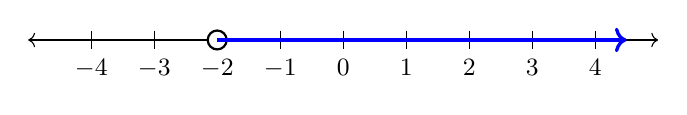
\begin{tikzpicture}[scale=0.8]
\draw[<->] (-5,0) -- (5,0);
\foreach \x in {-4,-3,-2,-1,0,1,2,3,4}
    \draw (\x,0.15) -- (\x,-0.15) node[below] {\small $\x$};
% Open circle at -2, arrow to the right
\draw[fill=white, thick] (-2,0) circle (0.15);
\draw[->, very thick, blue] (-2,0) -- (4.5,0);
\end{tikzpicture}
\end{center}

\vspace{1.5cm}
\end{questionbox}

\vspace{0.3cm}

%% Question 6
\begin{questionbox}
\textbf{Question 6} (1 mark)

Make $r$ the subject of the formula: \quad $A = \pi r^2$

\vspace{2.5cm}
\end{questionbox}

\vspace{0.3cm}

%% Question 7
\begin{questionbox}
\textbf{Question 7} (2 marks)

Make $x$ the subject of the formula: \quad $\displaystyle y = \frac{ax + b}{c}$

\vspace{3cm}
\end{questionbox}

\newpage

%% Question 8 - VISUAL: Two lines graph - find intersection
\begin{questionbox}
\textbf{Question 8} (2 marks)

The graph shows two lines $L_1$ and $L_2$.

\begin{center}
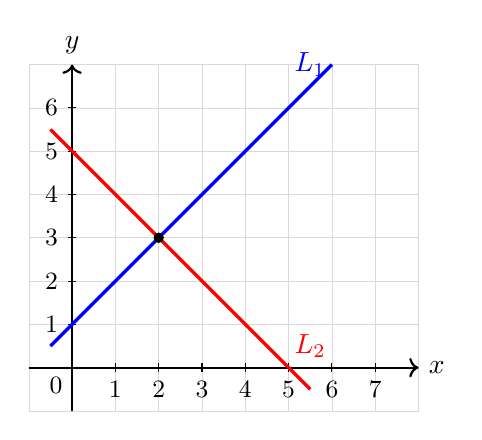
\begin{tikzpicture}[scale=0.55]
% Grid
\draw[gray!30, very thin] (-1,-1) grid (8,7);
% Axes
\draw[->, thick] (-1,0) -- (8,0) node[right] {$x$};
\draw[->, thick] (0,-1) -- (0,7) node[above] {$y$};
% Axis labels
\foreach \x in {1,2,3,4,5,6,7}
    \draw (\x,0.1) -- (\x,-0.1) node[below] {\small $\x$};
\foreach \y in {1,2,3,4,5,6}
    \draw (0.1,\y) -- (-0.1,\y) node[left] {\small $\y$};
\node[below left] at (0,0) {\small $0$};

% Line 1: y = x + 1 (passes through (0,1) and (5,6))
\draw[blue, very thick] (-0.5,0.5) -- (6,7);
\node[blue] at (5.5,7) {$L_1$};

% Line 2: y = -x + 5 (passes through (0,5) and (5,0))
\draw[red, very thick] (-0.5,5.5) -- (5.5,-0.5);
\node[red] at (5.5,0.5) {$L_2$};

% Intersection point at (2,3)
\fill (2,3) circle (0.12);
\end{tikzpicture}
\end{center}

\textbf{a.} Write down the equations of lines $L_1$ and $L_2$. (1 mark)

\vspace{2cm}

\textbf{b.} State the coordinates of the point of intersection. (1 mark)

\vspace{1.5cm}
\end{questionbox}

\vspace{0.3cm}

%% Question 9
\begin{questionbox}
\textbf{Question 9} (2 marks)

Solve the following pair of simultaneous equations using the \textbf{substitution} method:

\[
\begin{cases}
y = 2x - 1 \\
3x + y = 14
\end{cases}
\]

\vspace{4cm}
\end{questionbox}

\newpage

%% Question 10
\begin{questionbox}
\textbf{Question 10} (2 marks)

Solve the following pair of simultaneous equations using the \textbf{elimination} method:

\[
\begin{cases}
2x + 3y = 12 \\
4x - 3y = 6
\end{cases}
\]

\vspace{4cm}
\end{questionbox}

\vspace{0.3cm}

%% Question 11
\begin{questionbox}
\textbf{Question 11} (2 marks)

Solve the simultaneous equations:

\[
\begin{cases}
3x - 2y = 7 \\
x + 4y = -2
\end{cases}
\]

\vspace{4.5cm}
\end{questionbox}

\newpage

%% Question 12
\begin{questionbox}
\textbf{Question 12} (2 marks)

Solve the inequality and represent the solution on a number line:

\[ 3x + 5 > 14 \]

\vspace{2cm}

\begin{center}
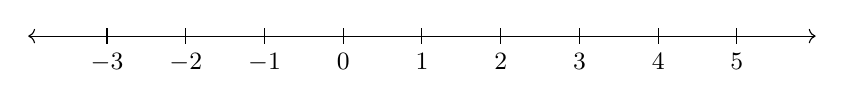
\begin{tikzpicture}
\draw[<->] (-4,0) -- (6,0);
\foreach \x in {-3,-2,-1,0,1,2,3,4,5}
    \draw (\x,0.1) -- (\x,-0.1) node[below] {\small $\x$};
\end{tikzpicture}
\end{center}

\vspace{1cm}
\end{questionbox}

\vspace{0.3cm}

%% Question 13
\begin{questionbox}
\textbf{Question 13} (2 marks)

Solve the inequality: \quad $\displaystyle \frac{x - 4}{2} \leq 3$

\vspace{3cm}
\end{questionbox}

\vspace{0.3cm}

%% Question 14
\begin{questionbox}
\textbf{Question 14} (2 marks)

Solve the inequality: \quad $-2x + 7 < 13$

\vspace{3cm}
\end{questionbox}

\newpage

%% Question 15 - VISUAL: Rectangle with expressions
\begin{questionbox}
\textbf{Question 15} (3 marks)

The diagram shows a rectangle with dimensions given in centimetres.

\begin{center}
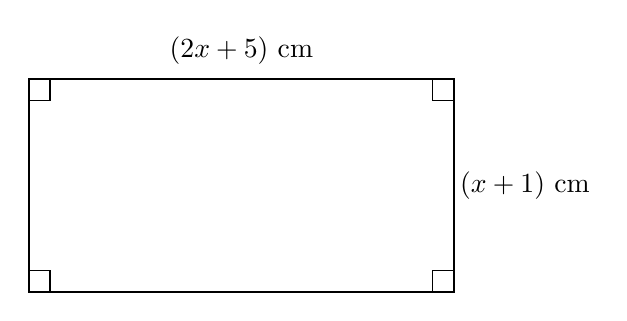
\begin{tikzpicture}[scale=0.9]
% Rectangle
\draw[thick] (0,0) rectangle (6,3);
% Labels
\node at (3,3.4) {$(2x + 5)$ cm};
\node at (7,1.5) {$(x + 1)$ cm};
% Right angle marks
\draw (0.3,0) -- (0.3,0.3) -- (0,0.3);
\draw (5.7,0) -- (5.7,0.3) -- (6,0.3);
\draw (0.3,3) -- (0.3,2.7) -- (0,2.7);
\draw (5.7,3) -- (5.7,2.7) -- (6,2.7);
\end{tikzpicture}
\end{center}

\textbf{a.} Write an expression for the perimeter of the rectangle. (1 mark)

\vspace{2cm}

\textbf{b.} If the perimeter is 54 cm, find the value of $x$. (1 mark)

\vspace{2.5cm}

\textbf{c.} Hence, find the area of the rectangle. (1 mark)

\vspace{2cm}
\end{questionbox}

\vspace{0.3cm}

%% Question 16
\begin{questionbox}
\textbf{Question 16} (2 marks)

The formula for converting temperature from Celsius ($C$) to Fahrenheit ($F$) is:
\[ F = \frac{9C}{5} + 32 \]

\textbf{a.} Convert $25^\circ$C to Fahrenheit. (1 mark)

\vspace{2cm}

\textbf{b.} Make $C$ the subject of the formula. (1 mark)

\vspace{2.5cm}
\end{questionbox}

\newpage

%% Question 17 - VISUAL: Triangle with perimeter
\begin{questionbox}
\textbf{Question 17} (3 marks)

The diagram shows an isosceles triangle with sides as labelled.

\begin{center}
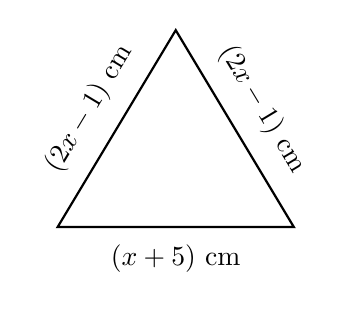
\begin{tikzpicture}[scale=1]
% Triangle
\draw[thick] (0,0) -- (3,0) -- (1.5,2.5) -- cycle;
% Labels
\node at (1.5,-0.4) {$(x + 5)$ cm};
\node[rotate=59] at (0.4,1.5) {$(2x - 1)$ cm};
\node[rotate=-59] at (2.6,1.5) {$(2x - 1)$ cm};
\end{tikzpicture}
\end{center}

\textbf{a.} Write an expression for the perimeter of the triangle. (1 mark)

\vspace{1.5cm}

\textbf{b.} If the perimeter is 38 cm, find the value of $x$. (1 mark)

\vspace{2.5cm}

\textbf{c.} Find the length of each side of the triangle. (1 mark)

\vspace{2cm}
\end{questionbox}

\vspace{0.3cm}

%% Question 18
\begin{questionbox}
\textbf{Question 18} (3 marks)

A phone plan charges a \$30 monthly fee plus \$0.15 per minute for calls.

\textbf{a.} Write an equation for the total monthly cost $C$ in terms of the number of minutes $m$ used. (1 mark)

\vspace{1.5cm}

\textbf{b.} If Sarah's bill was \$52.50, how many minutes did she use? (1 mark)

\vspace{2cm}

\textbf{c.} Another plan charges \$45 monthly with \$0.10 per minute. For how many minutes would both plans cost the same? (1 mark)

\vspace{2.5cm}
\end{questionbox}

\newpage

%% Question 19
\begin{questionbox}
\textbf{Question 19} (4 marks)

At a cinema, adult tickets cost \$18 and child tickets cost \$12.

A group bought 15 tickets in total and paid \$222.

\textbf{a.} Let $a$ be the number of adult tickets. Write an expression for the number of child tickets. (1 mark)

\vspace{1.5cm}

\textbf{b.} Write an equation for the total cost. (1 mark)

\vspace{1.5cm}

\textbf{c.} Solve the equation to find the number of adult and child tickets purchased. (2 marks)

\vspace{3cm}
\end{questionbox}

\newpage

% Section B
\section*{\underline{Section B: Extended Response Questions} {\color{gray}(14 Marks)}}

\vspace{0.5cm}

%% Question 20 (Extended) - VISUAL: Graph with two lines
\begin{questionbox}
\textbf{Question 20} (6 marks)

Two car rental companies offer the following rates:

\textbf{Company A:} \$50 per day plus \$0.20 per kilometre\\
\textbf{Company B:} \$80 per day plus \$0.10 per kilometre

\textbf{a.} Write an equation for the daily cost $C_A$ of renting from Company A in terms of kilometres $k$ travelled. (1 mark)

\vspace{1.5cm}

\textbf{b.} Write an equation for the daily cost $C_B$ of renting from Company B in terms of kilometres $k$ travelled. (1 mark)

\vspace{1.5cm}

\textbf{c.} On the axes below, sketch both cost equations. Label each line clearly. (2 marks)

\begin{center}
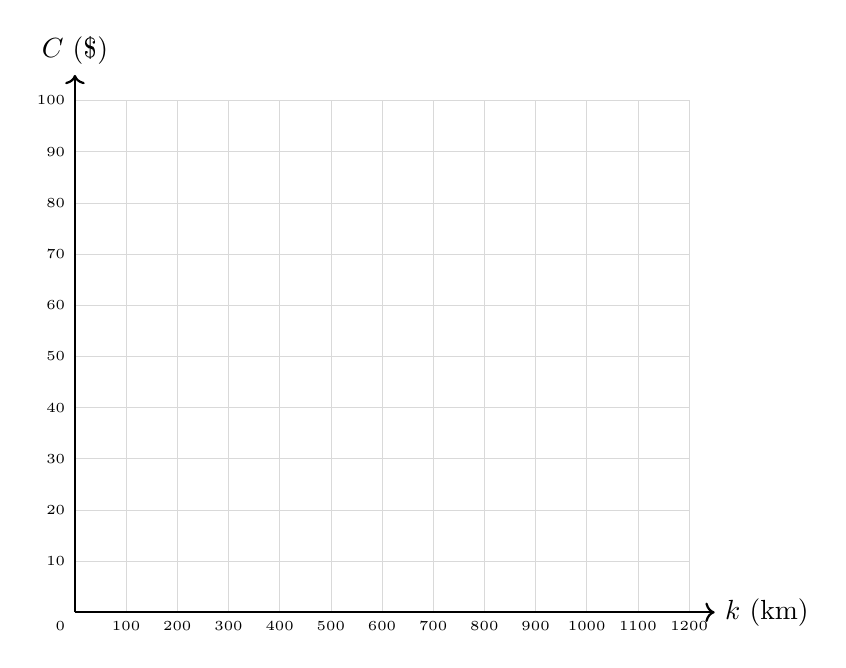
\begin{tikzpicture}[scale=0.65]
% Grid
\draw[gray!30, very thin] (0,0) grid (12,10);
% Axes
\draw[->, thick] (0,0) -- (12.5,0) node[right] {$k$ (km)};
\draw[->, thick] (0,0) -- (0,10.5) node[above] {$C$ (\$)};
% Axis labels
\foreach \x in {1,2,3,4,5,6,7,8,9,10,11,12}
    \node[below] at (\x,0) {\tiny $\x00$};
\foreach \y in {1,2,3,4,5,6,7,8,9,10}
    \node[left] at (0,\y) {\tiny $\y0$};
\node[below left] at (0,0) {\tiny $0$};
\end{tikzpicture}
\end{center}

\textbf{d.} For what distance would both companies charge the same amount? (1 mark)

\vspace{2cm}

\textbf{e.} If you plan to drive 400 km in one day, which company offers the better deal? Justify your answer. (1 mark)

\vspace{2.5cm}
\end{questionbox}

\newpage

%% Question 21 (Extended) - VISUAL: Paddock diagram
\begin{questionbox}
\textbf{Question 21} (8 marks)

A farmer has 120 metres of fencing to enclose a rectangular paddock. One side of the paddock is against an existing wall, so fencing is only needed for three sides.

Let $x$ metres be the length of the side perpendicular to the wall.

\begin{center}
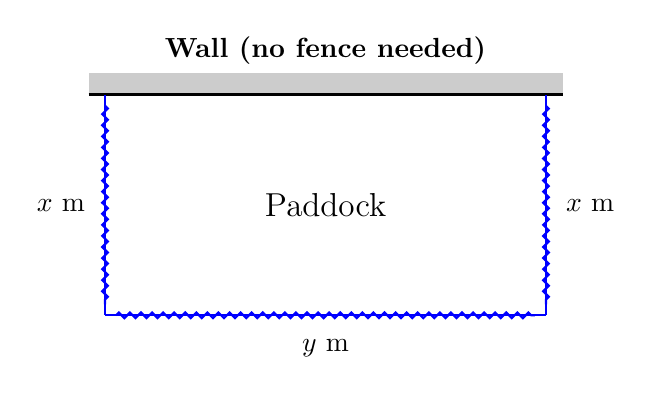
\begin{tikzpicture}[scale=0.7]
% Wall
\fill[gray!40] (-0.3,0) rectangle (8.3,0.4);
\draw[very thick] (-0.3,0) -- (8.3,0);
\node at (4,0.8) {\textbf{Wall (no fence needed)}};

% Rectangle
\draw[thick, blue] (0,0) -- (0,-4);
\draw[thick, blue] (0,-4) -- (8,-4);
\draw[thick, blue] (8,-4) -- (8,0);

% Labels
\node at (-0.8,-2) {$x$ m};
\node at (8.8,-2) {$x$ m};
\node at (4,-4.6) {$y$ m};

% Fence markers
\draw[thick, blue, decorate, decoration={zigzag, segment length=4pt, amplitude=1pt}] (0,-0.2) -- (0,-3.8);
\draw[thick, blue, decorate, decoration={zigzag, segment length=4pt, amplitude=1pt}] (8,-0.2) -- (8,-3.8);
\draw[thick, blue, decorate, decoration={zigzag, segment length=4pt, amplitude=1pt}] (0.2,-4) -- (7.8,-4);

% Area label
\node at (4,-2) {\large Paddock};
\end{tikzpicture}
\end{center}

\textbf{a.} Write an expression for the total length of fencing in terms of $x$ and $y$. (1 mark)

\vspace{1.5cm}

\textbf{b.} Given that the farmer uses all 120 m of fencing, write an expression for $y$ in terms of $x$. (1 mark)

\vspace{2cm}

\textbf{c.} Write an expression for the area $A$ of the paddock in terms of $x$ only. (1 mark)

\vspace{2cm}

\textbf{d.} If the farmer wants the paddock to have an area of 1600 m$^2$, form an equation and solve it to find the possible values of $x$. (3 marks)

\vspace{5cm}

\textbf{e.} State both possible sets of dimensions for the paddock. (2 marks)

\vspace{3cm}
\end{questionbox}

\newpage

% Answer Key (separate page)
\section*{ANSWER KEY}

\subsection*{Section A: Short Answer Questions}

\begin{enumerate}
\item $x = 6$
\item $x = -12$
\item $x = 9$
\item $x = 7$
\item $x > -2$
\item $r = \sqrt{\dfrac{A}{\pi}}$ (or $r = \pm\sqrt{\dfrac{A}{\pi}}$)
\item $x = \dfrac{cy - b}{a}$
\item (a) $L_1: y = x + 1$, \; $L_2: y = -x + 5$ \quad (b) $(2, 3)$
\item $x = 3$, $y = 5$
\item $x = 3$, $y = 2$
\item $x = \dfrac{12}{7}$, $y = -\dfrac{13}{14}$
\item $x > 3$ (open circle at 3, arrow right)
\item $x \leq 10$
\item $x > -3$
\item (a) $P = 2(2x+5) + 2(x+1) = 6x + 12$ \quad (b) $x = 7$ \quad (c) Area = $19 \times 8 = 152$ cm$^2$
\item (a) $77^\circ$F \quad (b) $C = \dfrac{5(F - 32)}{9}$
\item (a) $P = (2x-1) + (2x-1) + (x+5) = 5x + 3$ \quad (b) $x = 7$ \quad (c) Two sides of 13 cm, base of 12 cm
\item (a) $C = 30 + 0.15m$ \quad (b) 150 minutes \quad (c) 300 minutes
\item (a) $15 - a$ \quad (b) $18a + 12(15-a) = 222$ \quad (c) 7 adult, 8 child tickets
\end{enumerate}

\subsection*{Section B: Extended Response Questions}

\textbf{Question 20:}
\begin{enumerate}[label=(\alph*)]
\item $C_A = 50 + 0.20k$
\item $C_B = 80 + 0.10k$
\item Graph: $C_A$ starts at $(0, 50)$ with gradient $0.20$; $C_B$ starts at $(0, 80)$ with gradient $0.10$; lines intersect at $(300, 110)$
\item $k = 300$ km (where $50 + 0.20k = 80 + 0.10k$)
\item At 400 km: $C_A = \$130$, $C_B = \$120$. Company B is cheaper by \$10.
\end{enumerate}

\vspace{0.3cm}

\textbf{Question 21:}
\begin{enumerate}[label=(\alph*)]
\item Total fencing $= 2x + y$
\item $2x + y = 120 \Rightarrow y = 120 - 2x$
\item $A = x \times y = x(120 - 2x) = 120x - 2x^2$
\item $120x - 2x^2 = 1600$\\
$2x^2 - 120x + 1600 = 0$\\
$x^2 - 60x + 800 = 0$\\
$(x - 20)(x - 40) = 0$\\
$x = 20$ or $x = 40$
\item When $x = 20$: $y = 120 - 40 = 80$ m $\Rightarrow$ Dimensions: 20 m $\times$ 80 m\\
When $x = 40$: $y = 120 - 80 = 40$ m $\Rightarrow$ Dimensions: 40 m $\times$ 40 m
\end{enumerate}

\end{document}
